\begin{anexos}
	
	
	
	
	\begin{figure}[H]
		\centering
		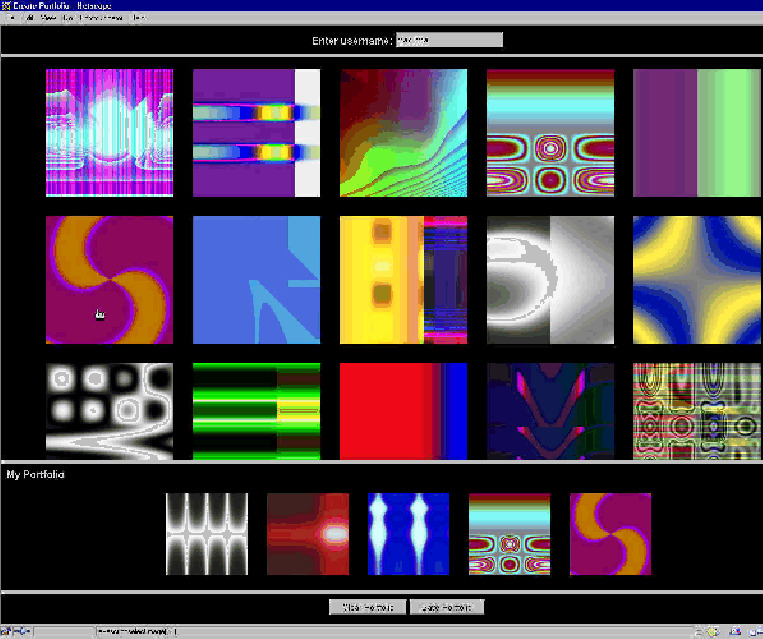
\includegraphics[width=0.5\linewidth]{Deja-Vu.jpg}
		\anexofigurecaption{Selección de portafolio. Fuente: \cite{dhamija2000deja}}
		\label{figure:deja-vu}
	\end{figure}


\begin{figure}[H]
	\centering
	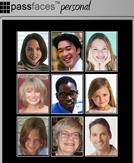
\includegraphics[width=0.3\linewidth]{3.jpg}
	\anexofigurecaption{Sistema PassFaces. Fuente: \cite{inproceedings}}
	\label{passfaces}
\end{figure}

\begin{figure}[H]
	\centering
	\begin{minipage}{0.5\linewidth}  % Tercer cuadrado, 48% del ancho de línea
		\centering
		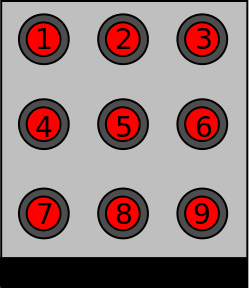
\includegraphics[width=0.7\linewidth]{0.png} % Imagen 3
	\end{minipage}%
	\hfill
	\begin{minipage}{0.5\linewidth} % Cuarto cuadrado, 48% del ancho de línea
		\centering
		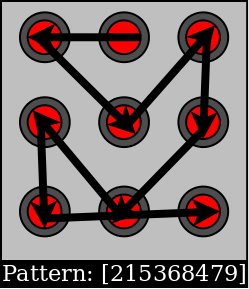
\includegraphics[width=0.7\linewidth]{1.png} % Imagen 4
	\end{minipage}
	\anexofigurecaption{Funcionamiento de un patrón de desbloqueo. Fuente: \cite{aviv2010smudge}}
	\label{android-pattern}
\end{figure}


\begin{figure}[H]
	\begin{minipage}{0.5\linewidth}  % Primer cuadrado, 48% del ancho de línea
		\centering
		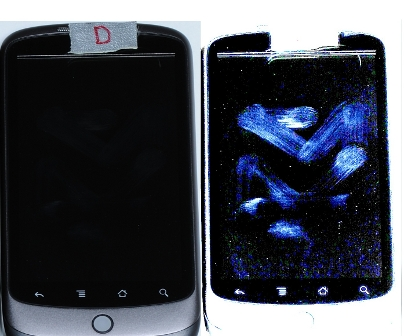
\includegraphics[width=\linewidth]{13.jpg} % Imagen 1
	\end{minipage}%
	\hfill
	\begin{minipage}{0.5\linewidth}  % Segundo cuadrado, 48% del ancho de línea
		\centering
		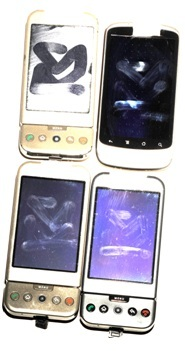
\includegraphics[width=0.5\linewidth]{9.jpg} % Imagen 2
	\end{minipage} % Espacio vertical entre filas

	\anexofigurecaption{Grasa en pantalla usada en los ataques de smudge. Fuente: \cite{aviv2010smudge}}
		\label{smudge-screen}
\end{figure} 

\begin{figure}[H]
	\centering
	\begin{minipage}{0.5\linewidth}  % Tercer cuadrado, 48% del ancho de línea
		\centering
		
\includegraphics[width=0.7\linewidth]{mouse.png} % Imagen 3
		\caption{Dibujado 6 veces usando el mouse. Fuente: \cite{lin2009free}}
		\label{free-draw-train-mouse}
	\end{minipage}%
	\hfill
	\begin{minipage}{0.5\linewidth} % Cuarto cuadrado, 48% del ancho de línea
		\centering
		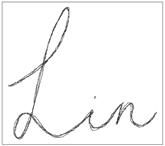
\includegraphics[width=0.7\linewidth]{stylus.png} % Imagen 4
		\caption{Dibujado 6 veces usando stylus. Fuente: \cite{lin2009free}}
		\label{free-draw-train-stylus}
	\end{minipage}
	
		\centering
	\begin{minipage}{0.48\linewidth}  % Tercer cuadrado, 48% del ancho de línea
		\centering
		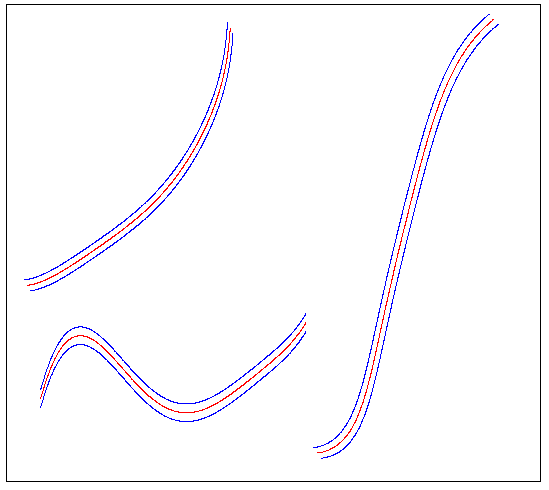
\includegraphics[width=0.9\linewidth]{polinomial.png} % Imagen 3
		\caption{Valores predichos e intervalos de predicción generados por el modelo de regresión polinomial. Fuente: \cite{lin2009free}}
		\label{free-form-draw-polinomial}
	\end{minipage}%
	\hfill
	\begin{minipage}{0.48\linewidth} % Cuarto cuadrado, 48% del ancho de línea
		\centering
		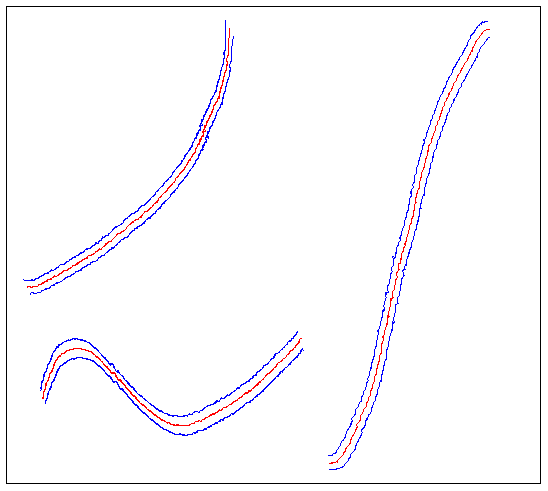
\includegraphics[width=0.9\linewidth]{b-spline.png} % Imagen 4
		\caption{Valores predichos e intervalos de predicción generados por el modelo de regresión B-spline. Fuente: \cite{lin2009free}}
		\label{free-form-draw-spline}
	\end{minipage}
	\anexofigurecaption{Valores predichos e intervalos de predicción generados por los modelos de regresi\'on. Fuente: \cite{lin2009free}}
	
\end{figure}




\begin{figure}[H]
	\centering
	\begin{minipage}{0.5\linewidth}  % Tercer cuadrado, 48% del ancho de línea
		\centering
		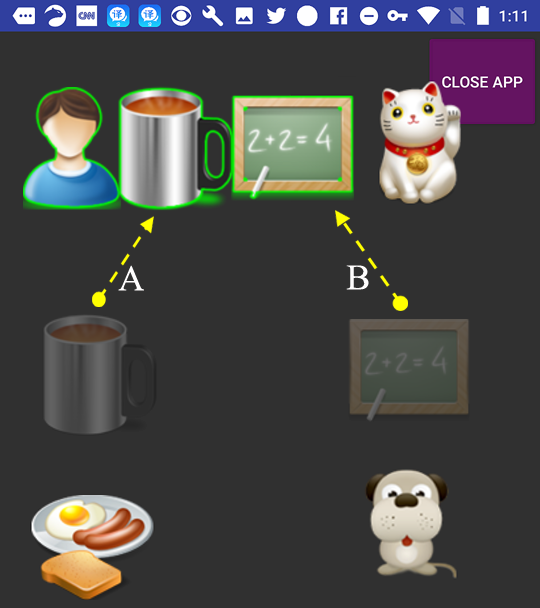
\includegraphics[width=0.8\linewidth]{semantoc-psw-2.png} % Imagen 3
		
	\end{minipage}%
	\hfill
	\begin{minipage}{0.5\linewidth} % Cuarto cuadrado, 48% del ancho de línea
		\centering
		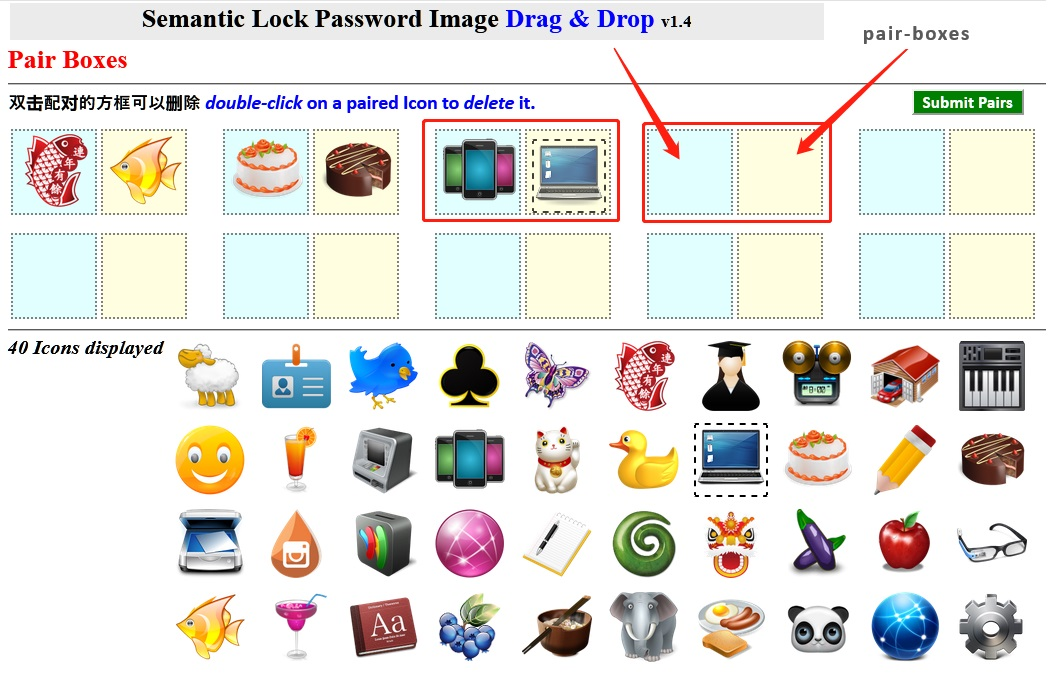
\includegraphics[width=0.8\linewidth]{semantic-psww1.jpg} % Imagen 4
		
	\end{minipage}
	\anexofigurecaption{Funcionamiento de Semantic Lock. Fuente: \cite{olade2023story}}
	\label{semantic-passw}
\end{figure}


\begin{figure}[H]
	 \centering
	\adjustbox{valign=b}{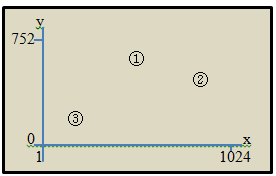
\includegraphics[width=0.8\linewidth]{pass-positions.png}} % valign=t para alinear la imagen en la parte superior
	\anexofigurecaption{Cálculo de hash de un punto Passpositions. Fuente: \cite{8320723}}
	\label{passpositions-example}
	
\end{figure}

\begin{figure}[H]
	\centering
	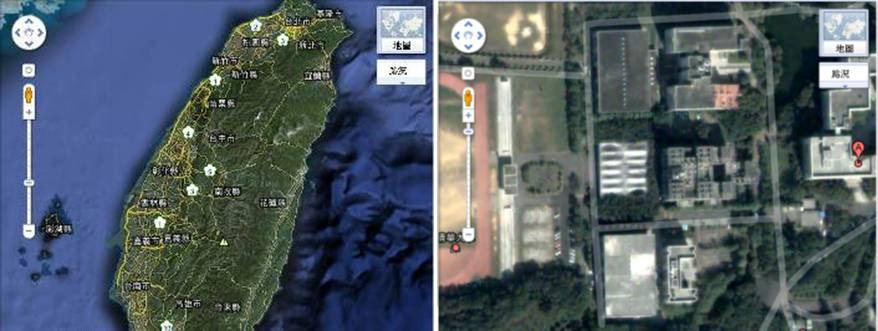
\includegraphics[width=0.5\linewidth]{pass maps2.jpg}
	\anexofigurecaption{Información del mapa en diferentes lugares y niveles de zoom. Fuente: \cite{10.1145/2414456.2414513}}
	\label{passmap}
\end{figure}

\begin{figure}[H]
	\begin{minipage}{0.5\linewidth}  % Primer cuadrado, 48% del ancho de línea
		\centering
		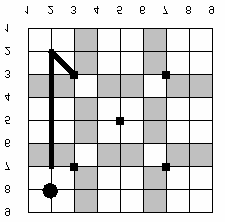
\includegraphics[width=\linewidth]{passgo1.png} % Imagen 1
	\end{minipage}%
	\hfill
	\begin{minipage}{0.5\linewidth}  % Segundo cuadrado, 48% del ancho de línea
		\centering
		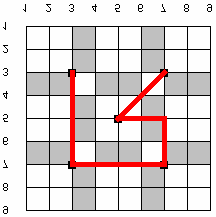
\includegraphics[width=\linewidth]{passgo2.png} % Imagen 2
	\end{minipage} % Espacio vertical entre filas
	\hfill
	\begin{minipage}{0.5\linewidth}  % Segundo cuadrado, 48% del ancho de línea
		\centering
		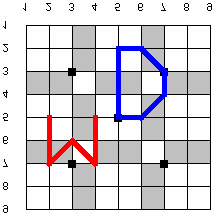
\includegraphics[width=\linewidth]{passgo3.png} % Imagen 2
	\end{minipage} % Espacio vertical entre filas
	\anexofigurecaption{Ejemplos de contraseñas usando Pass Go. Fuente: \cite{tao2008pass}}
	\label{go-passwords}
\end{figure} 



 \begin{figure}[H]
 	\begin{figure}[H]
 		\centering
 		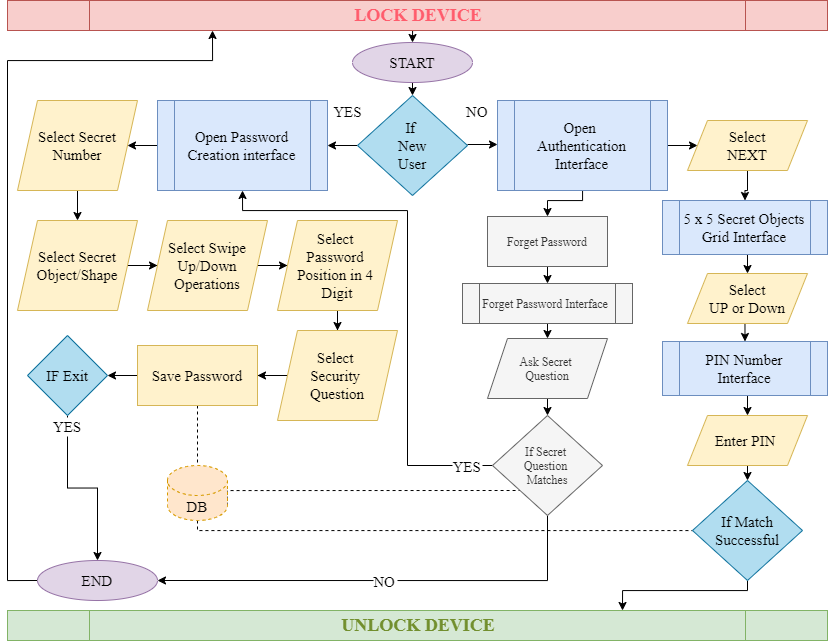
\includegraphics[width=0.6\linewidth]{grapin-proceso.png}
 		\caption{Proceso de autenticación \textit{Gra-Pin}. Fuente: \cite{kausar2022gra} }
 		\label{gra-pin}
 	\end{figure}
	\centering
	\begin{minipage}[b]{0.4\linewidth}  % Tercer cuadrado, 48% del ancho de línea
		\centering
		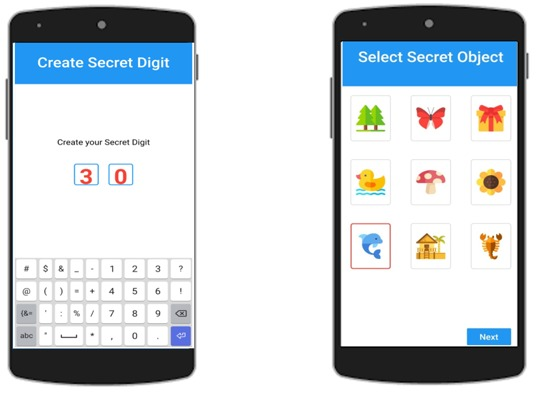
\includegraphics[width=\linewidth]{grapin-secret.jpg}
		\caption{Selección del número e imagen secretos. Fuente: \cite{kausar2022gra} }
	\end{minipage}%
	\hfill
	\begin{minipage}[b]{0.5\linewidth} % Cuarto cuadrado, 48% del ancho de línea
		\centering
		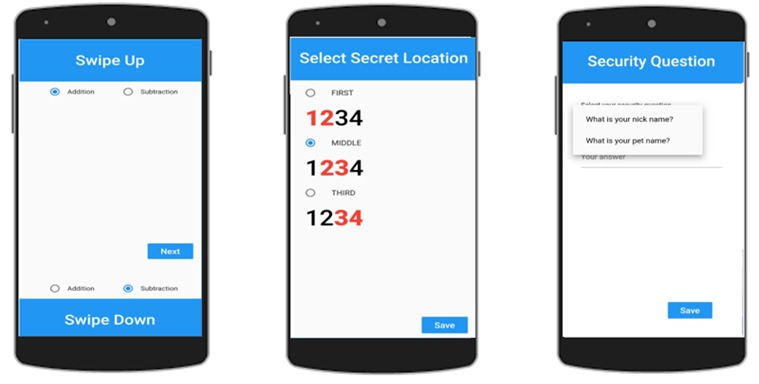
\includegraphics[width=\linewidth]{grapin-position.jpg}
		\caption{Selección de la operación y posición en el Pin de la clave. Fuente: \cite{kausar2022gra}  }          
	\end{minipage}
	\begin{minipage}[b]{0.4\linewidth} % Cuarto cuadrado, 48% del ancho de línea
		\centering
		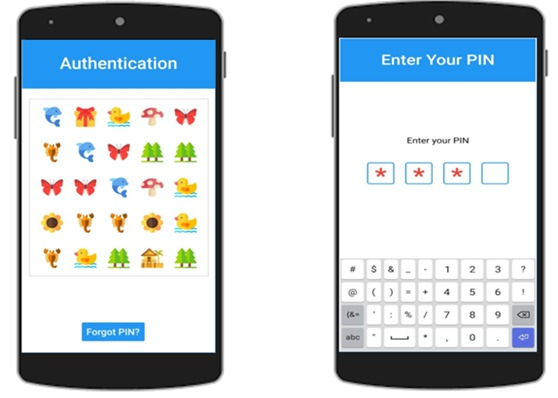
\includegraphics[width=\linewidth]{grapin-auth.jpg}
		\caption{Pantalla de autenticación. Fuente: \cite{kausar2022gra}}
		
	\end{minipage}
	\anexofigurecaption{Pantallas de autenticación de \textit{Gra Pin}. Fuente: \cite{kausar2022gra}}
	\label{gra-pin-screens}
\end{figure}




%capturas
\begin{figure}
	\begin{figure}[H]
		\centering
		\begin{minipage}[b]{0.48\linewidth}  % Tercer cuadrado, 48% del ancho de línea
			\centering
			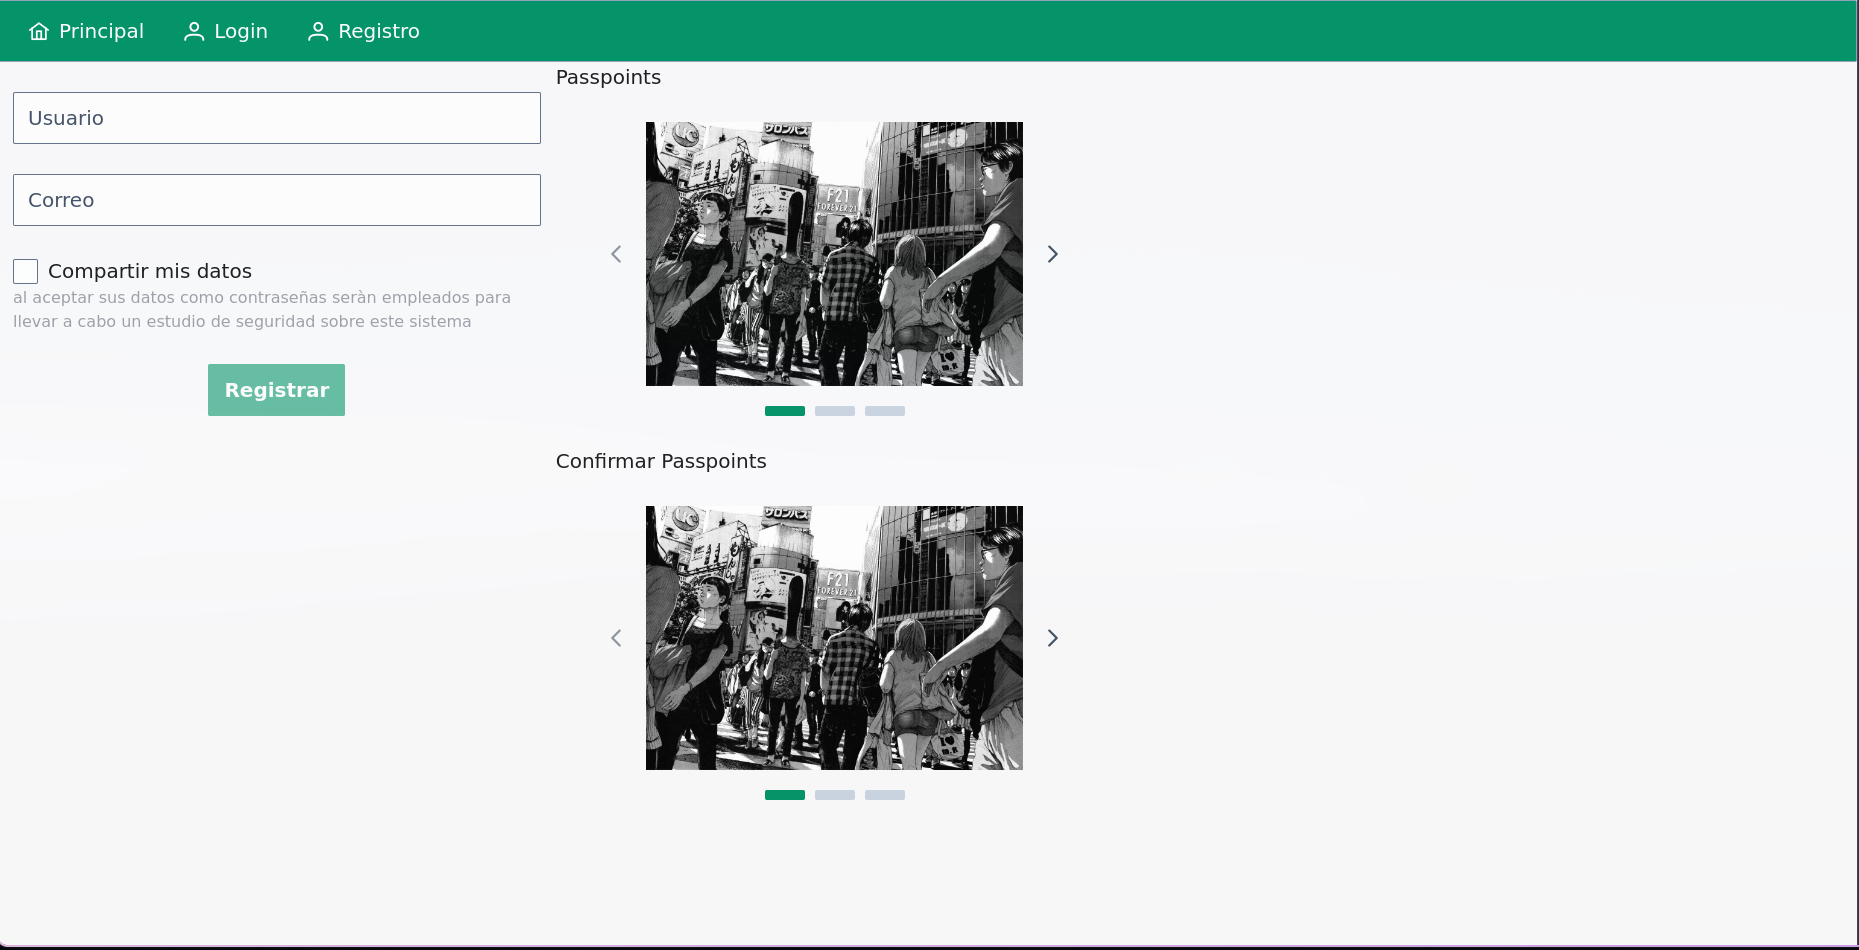
\includegraphics[width=\linewidth]{Graphics/capturas/registro-landscape.png}
			\caption{Pantalla de registro en vista escritorio }
			\label{register-screen}
		\end{minipage}%
		\hfill
		\begin{minipage}[b]{0.48\linewidth} % Cuarto cuadrado, 48% del ancho de línea
			\centering
			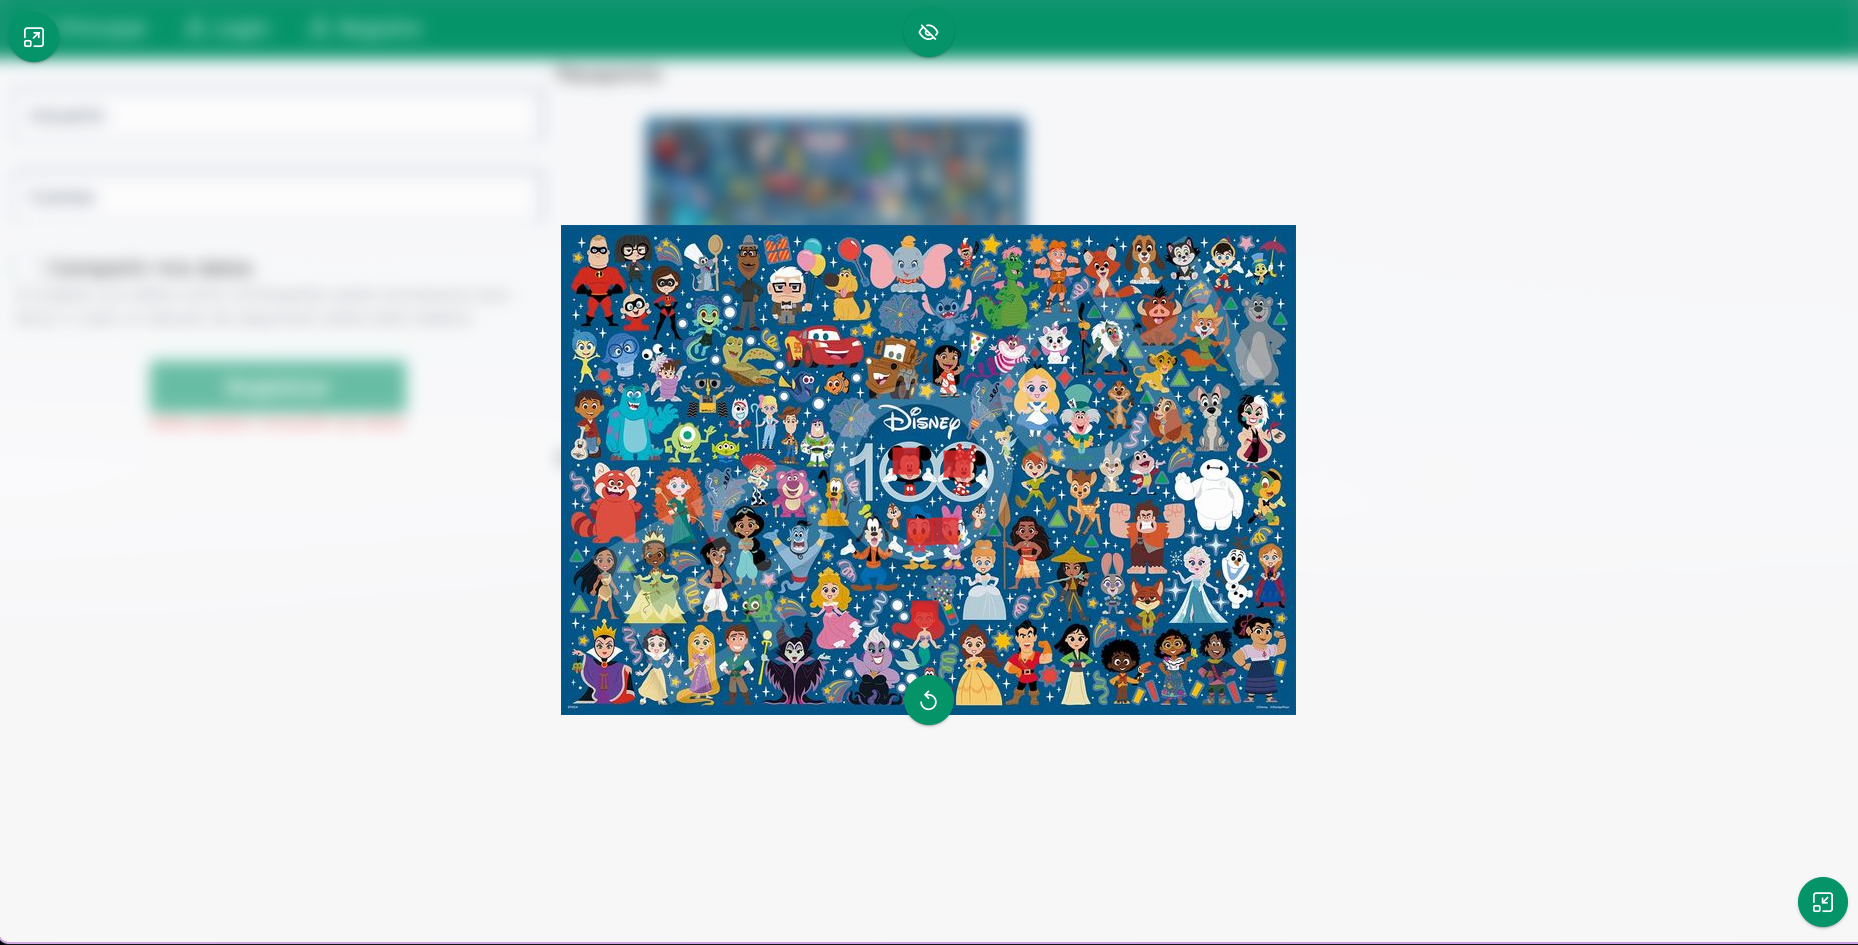
\includegraphics[width=\linewidth]{Graphics/capturas/fullscreen-password-selector.png}
			\caption{Selecci\'on de imagen y contrase\~na a pantalla completa }   
			\label{full-screen-password}       
		\end{minipage}
		
	\end{figure} 
	
	\begin{figure}[H]
		\centering
		\begin{minipage}[b]{0.48\linewidth}  % Tercer cuadrado, 48% del ancho de línea
			\centering
			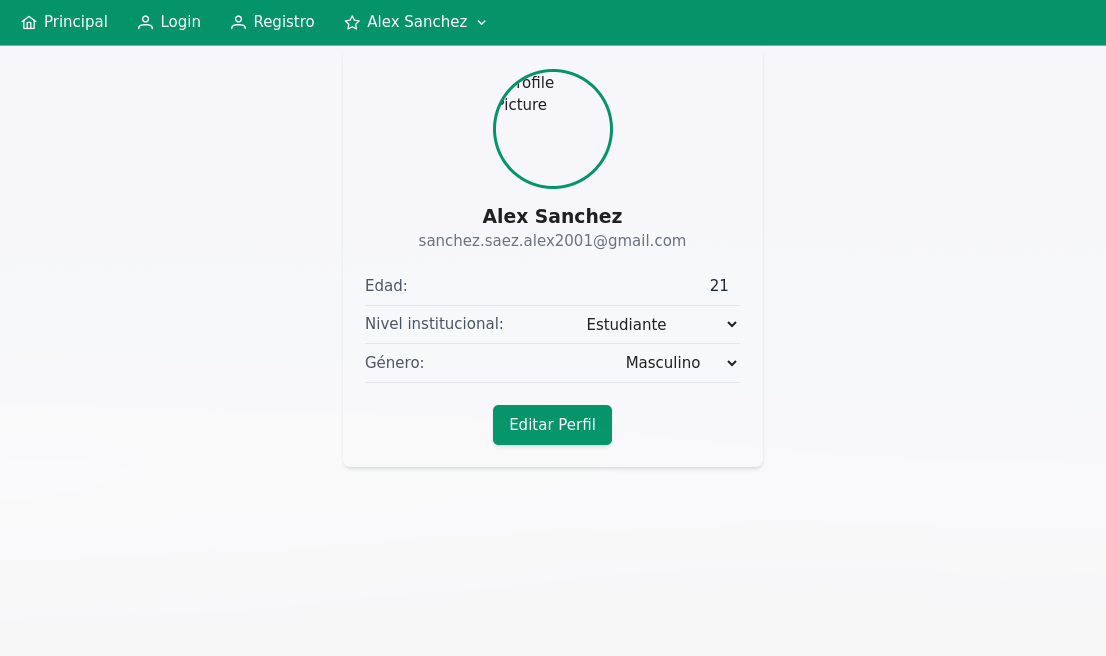
\includegraphics[width=\linewidth]{Graphics/capturas/profile.png}
			\caption{Perfil del usuario para recaudar informaci\'on }
			\label{user-profile} 
		\end{minipage}%
		\hfill
		\begin{minipage}[b]{0.48\linewidth} % Cuarto cuadrado, 48% del ancho de línea
			\centering
			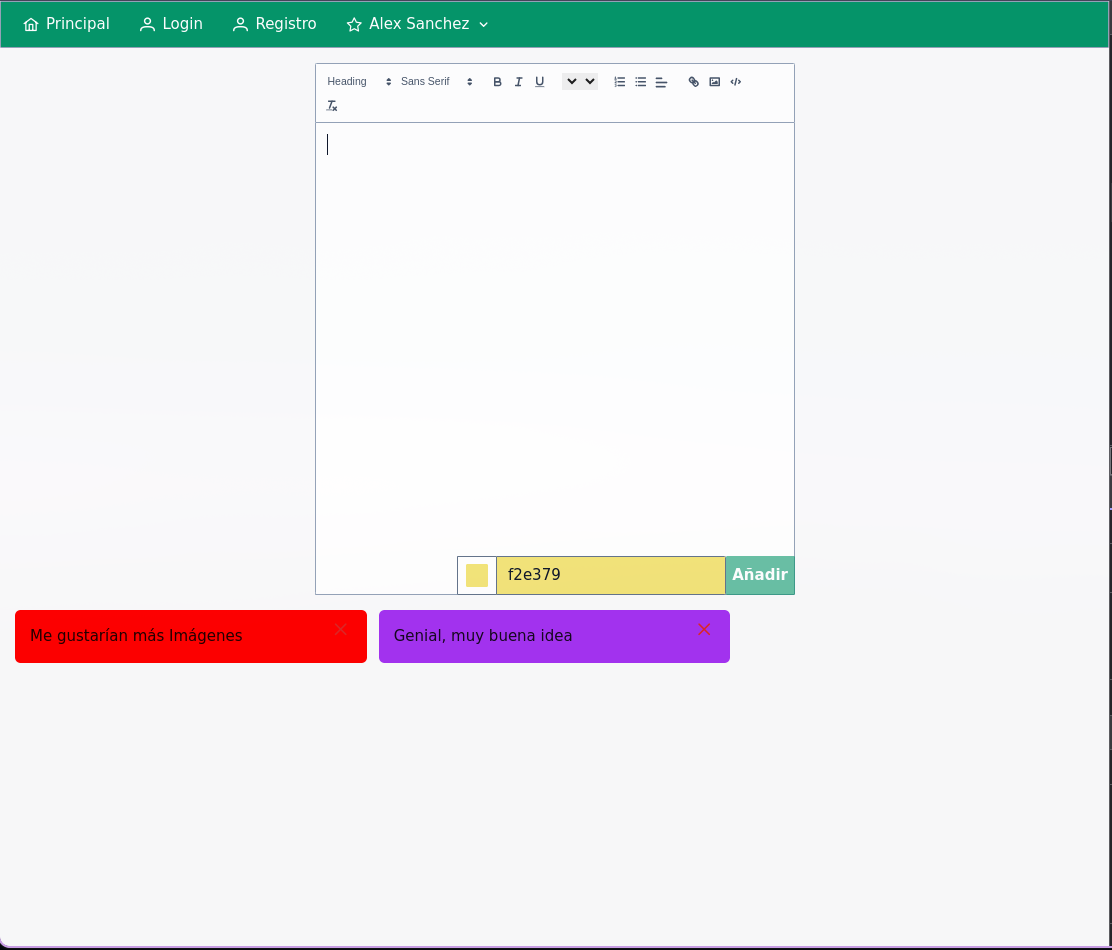
\includegraphics[width=\linewidth]{Graphics/capturas/notes.png}
			\caption{Vista de notas para dejar valoraciones } 
			\label{notes}          
		\end{minipage}
	\end{figure}
	
	\begin{figure}[H]
		\centering
		\begin{minipage}[b]{0.68\linewidth}  % Tercer cuadrado, 48% del ancho de línea
			\centering
			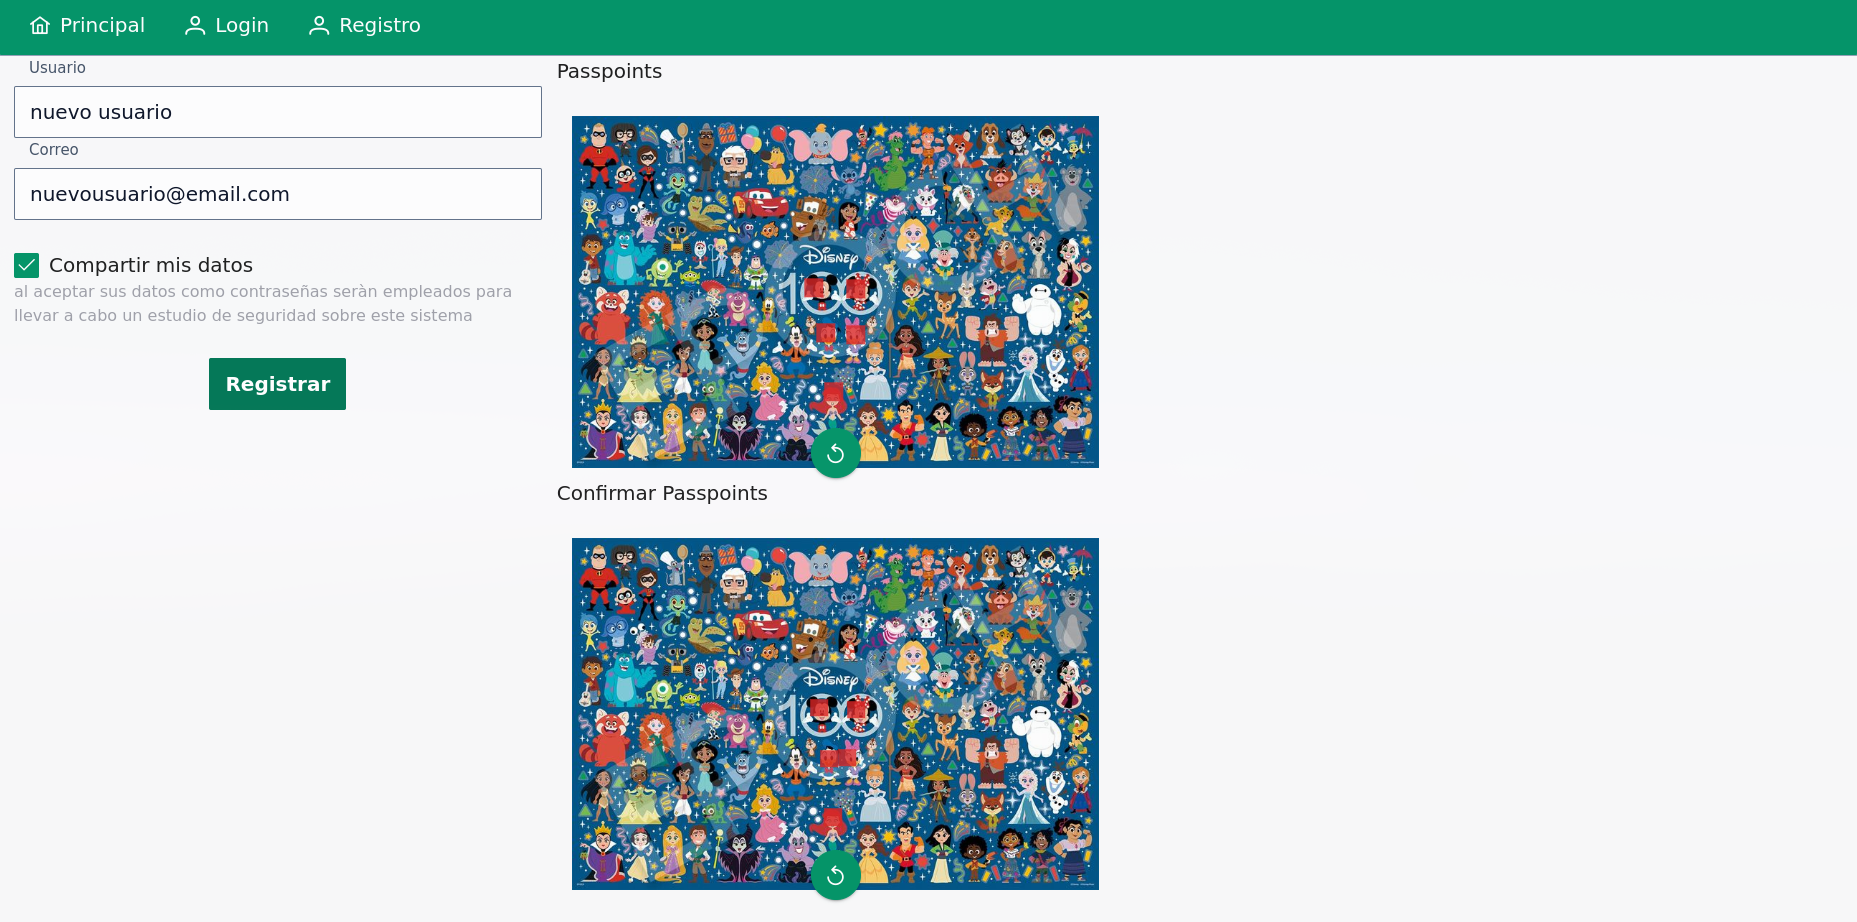
\includegraphics[width=\linewidth]{Graphics/capturas/full-screen disney-password.png}
			
		\end{minipage}%
		\hfill
		\begin{minipage}[b]{0.3\linewidth} % Cuarto cuadrado, 48% del ancho de línea
			\centering
			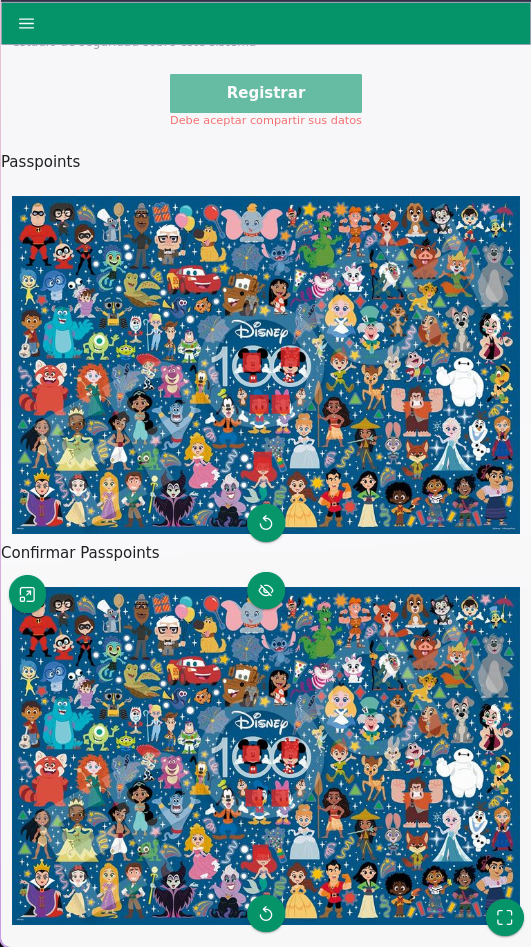
\includegraphics[width=\linewidth]{Graphics/capturas/password-mobile.png}
			
		\end{minipage}
		
		
		\caption{Misma contrase\~na en diferentes taman\~nos de pantalla }
		\label{screen-shapes-variety}
	\end{figure}
	
	\begin{figure}[H]
		\centering
		\begin{minipage}[b]{0.68\linewidth}  % Tercer cuadrado, 48% del ancho de línea
			\centering
			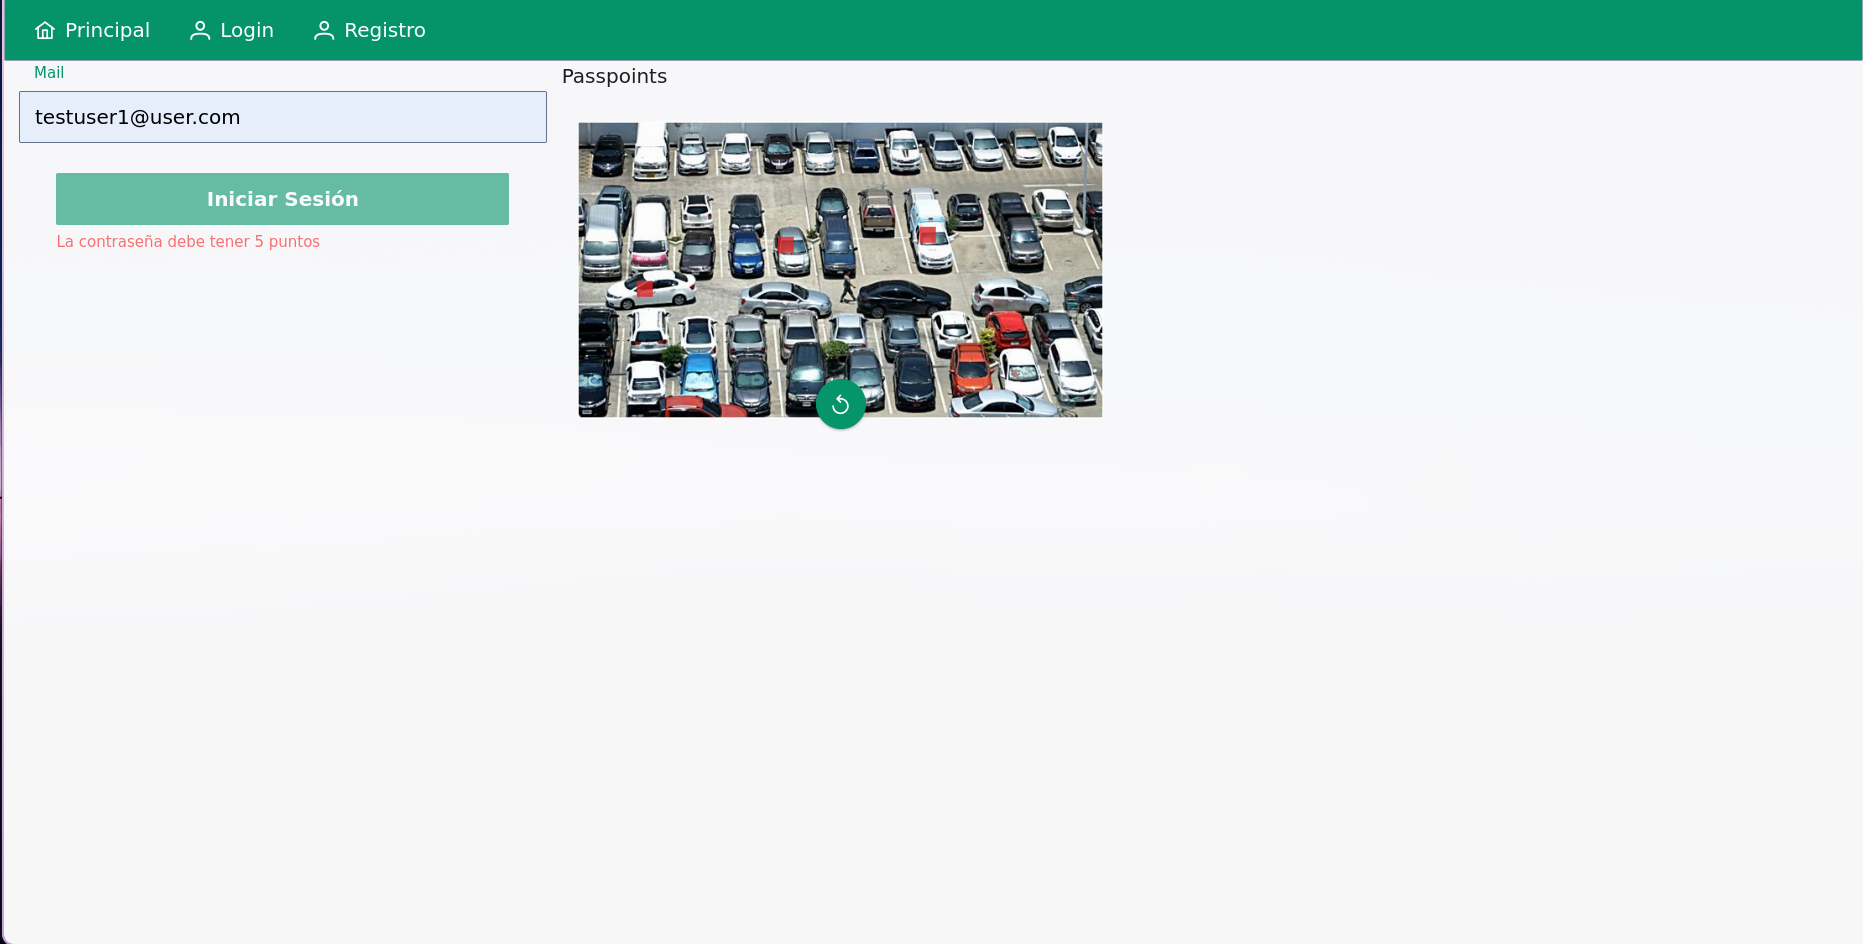
\includegraphics[width=\linewidth]{Graphics/capturas/cars-login-error-landscape.png}
			
		\end{minipage}%
		\hfill
		\begin{minipage}[b]{0.3\linewidth} % Cuarto cuadrado, 48% del ancho de línea
			\centering
			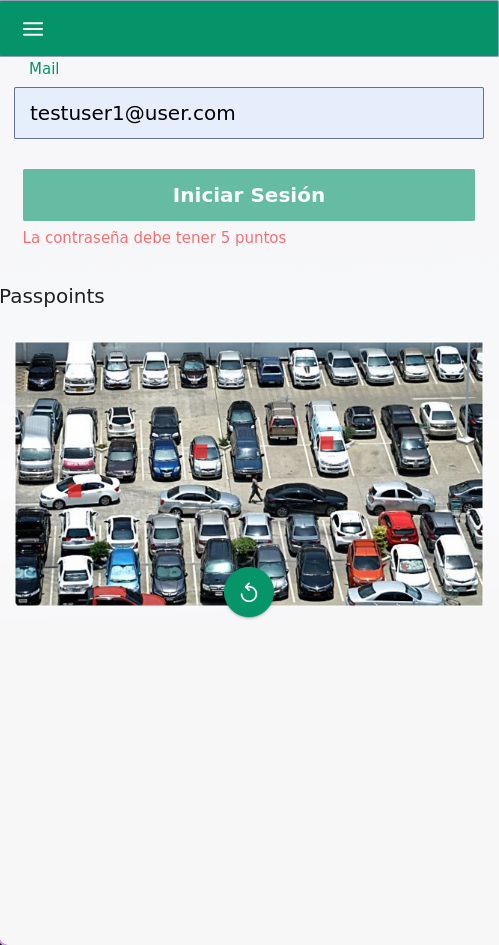
\includegraphics[width=\linewidth]{Graphics/capturas/login-error-mobile.png}
			
		\end{minipage}
		\caption{Misma contrase\~na incorrecta en diferentes taman\~nos de pantalla }
		\label{error-scans}
	\end{figure}
		\anexofigurecaption{Diferentes vistas de la aplicaci\'on}
\end{figure}




\end{anexos}
